\documentclass[border=2mm]{standalone}

\usepackage{tikz}

\usetikzlibrary{decorations.pathmorphing,patterns}

\begin{document}

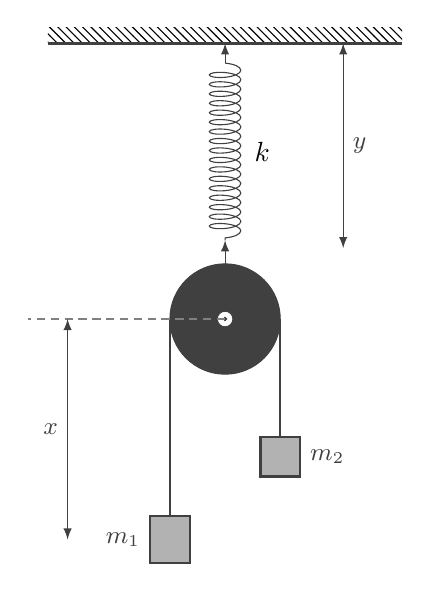
\begin{tikzpicture}[black!75]

\fill [pattern = north west lines] (-2.25,0) rectangle ++(4.5,.2);

\draw[thick] (-2.25,0) -- ++(4.5,0);

\draw[latex-] (0,0) -- ++(0,-0.25);

\draw[decoration={aspect=0.3, segment length=1.2mm, amplitude=2mm,coil},decorate] (0,-0.25) -- ++(0,-2.25) node[midway,right=0.25cm,black]{$k$};

\draw[latex-] (0,-2.5) -- ++(0,-0.3);

\draw[fill=black!75] (0,-3.5) circle(0.7cm);

\draw[fill=white] (0,-3.5) circle(0.1cm);

\draw[fill=black!75] (0,-3.5) circle(0.02cm);

\draw[thick,fill=gray!60] (0.7,-3.5) -- ++(0,-1.5) ++(-0.25,-0.5) rectangle ++(0.5,0.5)node[midway, right=0.25cm]{\small $m_2$} ;

\draw[thick,fill=gray!60] (-0.7,-3.5) -- ++(0,-2.5) ++(-0.25,-0.6) rectangle ++(0.5,0.6) node[midway, left=0.25cm]{\small $m_1$} ;

\draw[gray,densely dashed] (0,-3.5) -- ++ (-2.5,0);

\draw[latex-latex] (-2,-3.5) -- ++(0,-2.8)node[midway,left]{\small $x$};

\draw[latex-latex] (1.5,0) -- ++(0,-2.6)node[midway,right]{\small $y$};

\end{tikzpicture}

\end{document}